% Software Requirements Specification for Canteen Ordering System
\documentclass[11pt]{article}
\usepackage[margin=1in]{geometry}
\usepackage{hyperref}
\usepackage{url}
\usepackage{booktabs}
\usepackage{longtable}
\usepackage{tikz}
\usetikzlibrary{positioning}
\usepackage{graphicx}
\usepackage{enumitem}
\usepackage{titlesec}
\titleformat{\section}{\normalfont\Large\bfseries}{\thesection}{1em}{}
\titleformat{\subsection}{\normalfont\large\bfseries}{\thesubsection}{1em}{}
\title{Software Requirements Specification}
\author{Canteen Ordering and Management System}
\date{\today}

\begin{document}
\maketitle
\pagenumbering{roman}
\tableofcontents
\newpage
\pagenumbering{arabic}

\section{Introduction}
\subsection{Purpose}
This document defines the software requirements for the Canteen Ordering and Management System implemented in the provided repository. It is derived directly from the actual implementation of the mobile student application, the admin dashboard, and the FastAPI backend with MongoDB.

\subsection{Scope}
The system supports student-facing ordering, wallet-based and UPI payments, QR-based order verification, and administrative management of menu items, combos, inventory, orders, users, and wallet transactions.

\subsection{Definitions, Acronyms, and Abbreviations}
\begin{itemize}[nosep]
  \item JWT: JSON Web Token
  \item API: Application Programming Interface
  \item UPI: Unified Payments Interface
  \item UI: User Interface
  \item CRUD: Create, Read, Update, Delete
  \item RN: React Native
\end{itemize}

\subsection{References}
\begin{itemize}[nosep]
  \item \cite{fastapi}
  \item \cite{reactnative}
  \item \cite{mongodb}
  \item \cite{expo}
  \item \cite{typescript}
\end{itemize}

\subsection{Overview}
This SRS document describes the product perspective, system features, external interface requirements, and quality attributes of the implemented application. The system is divided into:
\begin{itemize}[nosep]
  \item Mobile student app built with Expo React Native.
  \item Admin dashboard built with React, TypeScript, Vite, and Tailwind.
  \item Backend implemented in FastAPI and MongoDB.
\end{itemize}

\section{Overall Description}
\subsection{Product Perspective}
The system is a three-tier architecture:
\begin{itemize}[nosep]
  \item Mobile client (\texttt{canteen-frontend}): student-facing ordering and wallet experience.
  \item Admin dashboard (\texttt{canteen-admin}): menu management, order management, inventory, and analytics.
  \item Backend service (\texttt{canteen-backend}): REST API, authentication, persistence, business logic, and QR verification.
\end{itemize}

\subsection{Product Functions}
Key implemented functions include:
\begin{itemize}[nosep]
  \item User authentication and session management via JWT tokens.
  \item Menu browsing with filtering, trending, featured, and specials endpoints.
  \item Combo browsing and management.
  \item Cart management and order creation.
  \item Wallet balance retrieval, history, PIN setup/change, and top-up.
  \item Checkout summary calculation.
  \item Payment processing for wallet and UPI.
  \item QR code generation and verification for order pickup.
  \item Admin order status updates and live order management.
  \item Admin CRUD operations for menu items, combos, and inventory.
\end{itemize}

\subsection{User Characteristics}
The system targets two user roles:
\begin{itemize}[nosep]
  \item Student users: authenticate, browse food, place orders, pay, view orders, and show QR codes.
  \item Admin users: authenticate to dashboard, manage orders, control menu/combo inventory, and monitor payments.
\end{itemize}

\subsection{Constraints}
The actual implementation includes the following constraints:
\begin{itemize}[nosep]
  \item Backend uses FastAPI with CORS configured to allow all origins for development.
  \item Mobile app uses a hard-coded backend base URL: \texttt{http://192.168.0.149:8000/api}.
  \item Authentication depends on JWT bearer tokens stored locally in AsyncStorage or localStorage.
  \item Admin RBAC is currently supported in dependencies but a demo fallback token \texttt{mock-jwt-token} is accepted.
\end{itemize}

\subsection{Assumptions and Dependencies}
The implementation depends on:
\begin{itemize}[nosep]
  \item MongoDB as the primary persistence layer.
  \item FastAPI backend hosted at the configured API base URL.
  \item Expo React Native runtime for the mobile client.
  \item React and Vite build chain for the admin dashboard.
\end{itemize}

\section{Specific Requirements}
\subsection{External Interface Requirements}
\subsubsection{User Interfaces}
The system supports two user interfaces:
\begin{itemize}[nosep]
  \item Student mobile UI implemented in \texttt{canteen-frontend/src/screens}, including \texttt{LoginScreen.js}, \texttt{MenuScreen.js}, \texttt{OrdersScreen.js}, and \texttt{QRScreen.js}.
  \item Admin web UI implemented in \texttt{canteen-admin/src/pages}, including \texttt{Login.tsx}, \texttt{LiveOrders.tsx}, \texttt{MenuManagement.tsx}, \texttt{ComboManagement.tsx}, \texttt{InventoryManagement.tsx}, \texttt{WalletDashboard.tsx}, and \texttt{ReportsAnalytics.tsx}.
\end{itemize}

\subsubsection{Hardware Interfaces}
The system assumes standard mobile device and web browser hardware. No specialized hardware interfaces are coded in the repository.

\subsubsection{Software Interfaces}
The backend exposes RESTful JSON endpoints documented in Section \ref{sec:api-reference}. The mobile and admin clients consume these APIs via Axios.

\subsubsection{Communications Interfaces}
All communication between clients and backend occurs over HTTP/HTTPS using bearer token authorization. The mobile app stores the JWT in AsyncStorage and attaches it to the \texttt{Authorization} header. The admin dashboard stores the token in localStorage.

\subsection{System Features}
\subsubsection{Authentication and Authorization}
\begin{itemize}[nosep]
  \item \textbf{Login}: \texttt{POST /api/auth/login} accepts credentials and returns a JWT token and user payload.
  \item \textbf{Registration}: \texttt{POST /api/auth/register} creates a new user.
  \item \textbf{Current user}: \texttt{GET /api/auth/me} returns authenticated user details.
  \item \textbf{Protected routes}: backend dependencies \texttt{get\_current\_user} and \texttt{get\_current\_admin} enforce JWT authentication.
\end{itemize}

\subsubsection{Menu Management}
\begin{itemize}[nosep]
  \item \texttt{GET /api/menu} lists menu items with optional filters for category, availability, vegetarian, trending, special, featured, and sorting.
  \item \texttt{GET /api/menu/trending}, \texttt{/menu/specials}, \texttt{/menu/featured} provide curated lists.
  \item \texttt{POST /api/menu}, \texttt{PATCH /api/menu/\{item\_id\}}, and \texttt{DELETE /api/menu/\{item\_id\}} allow admin CRUD operations.
\end{itemize}

\subsubsection{Combo Management}
\begin{itemize}[nosep]
  \item \texttt{GET /api/combos} returns combo bundles with pagination support.
  \item \texttt{GET /api/combos/trending}, \texttt{/api/combos/featured} highlight promotional bundles.
  \item \texttt{POST /api/combos}, \texttt{PATCH /api/combos/\{combo\_id\}}, \texttt{DELETE /api/combos/\{combo\_id\}} support admin combo lifecycle.
\end{itemize}

\subsubsection{Ordering and Checkout}
\begin{itemize}[nosep]
  \item \texttt{POST /api/orders} creates a new order from shopping cart payload.
  \item \texttt{GET /api/orders} lists the authenticated user's orders.
  \item \texttt{GET /api/orders/all} returns all orders for administrative review.
  \item \texttt{GET /api/orders/\{order\_id\}} retrieves order details.
  \item \texttt{GET /api/orders/\{order\_id\}/status} retrieves order status.
  \item \texttt{PATCH /api/orders/\{order\_id\}/status} updates order status.
  \item \texttt{POST /api/checkout/summary} computes checkout summaries and offerable totals.
\end{itemize}

\subsubsection{Wallet and Payment}
\begin{itemize}[nosep]
  \item \texttt{GET /api/wallet} retrieves wallet details.
  \item \texttt{GET /api/wallet/history} returns wallet transaction history.
  \item \texttt{POST /api/wallet/set-pin} and \texttt{PUT /api/wallet/change-pin} manage wallet PINs.
  \item \texttt{POST /api/wallet/add} adds balance to the wallet.
  \item \texttt{POST /api/payments/wallet-pay} processes wallet payments.
  \item \texttt{POST /api/payments/upi-pay} processes UPI payments.
  \item \texttt{GET /api/payments/history} returns the payment transaction history.
\end{itemize}

\subsubsection{Profile Management}
\begin{itemize}[nosep]
  \item \texttt{GET /api/profile} returns the current user's profile.
  \item \texttt{PUT /api/profile} updates user details.
\end{itemize}

\subsubsection{QR Order Verification}
\begin{itemize}[nosep]
  \item \texttt{GET /api/qr/orders/\{order\_id\}} generates QR payload for an order.
  \item \texttt{POST /api/qr/verify} validates QR data and returns order verification details.
\end{itemize}

\subsubsection{Inventory Management}
\begin{itemize}[nosep]
  \item \texttt{POST /api/inventory} creates inventory records.
  \item \texttt{GET /api/inventory} lists inventory items with pagination and search.
  \item \texttt{GET /api/inventory/\{id\}} retrieves a single inventory item.
  \item \texttt{PATCH /api/inventory/\{id\}} updates inventory stock.
  \item \texttt{DELETE /api/inventory/\{id\}} removes inventory records.
\end{itemize}

\subsection{Performance Requirements}
The system uses pagination on menu, combo, order, wallet history, and inventory endpoints to keep responses efficient. Client-side request timeouts are set to 10 seconds in the mobile app.

\subsection{Design Constraints}
\begin{itemize}[nosep]
  \item Backend architecture is implemented in Python/FastAPI with MongoDB.
  \item Mobile UI uses Expo-managed React Native and AsyncStorage.
  \item Admin dashboard is TypeScript-based and uses React Query for data fetching.
\end{itemize}

\subsection{Software System Attributes}
\begin{itemize}[nosep]
  \item \textbf{Security}: JWT authentication with bearer token header, and role-aware access control via backend dependencies.
  \item \textbf{Usability}: student app supports search, filters, and progressive loading states.
  \item \textbf{Maintainability}: separation of frontend service modules, admin API wrappers, and backend routers/services.
\end{itemize}

\subsection{Other Requirements}
The backend includes a health endpoint \texttt{GET /health} for basic availability checks.

\section{API Reference}
\label{sec:api-reference}
\subsection{Authentication}
\begin{longtable}{p{3.2cm} p{1.7cm} p{2.2cm} p{3.6cm} p{3.6cm} p{1.8cm} p{1.8cm}}
\toprule
Route & Method & Auth & Request Schema & Response Schema & Success & Error \\
\midrule
\endfirsthead
\toprule
Route & Method & Auth & Request Schema & Response Schema & Success & Error \\
\midrule
\endhead
\bottomrule
\endfoot

/api/auth/register & POST & No & \texttt{RegisterRequest} & \texttt{TokenResponse} & 201 Created & 400 Bad Request, 409 Conflict (duplicate email), 422 Validation Error \\

/api/auth/login & POST & No & \texttt{LoginRequest} & \texttt{TokenResponse} & 200 OK & 401 Unauthorized (incorrect credentials), 422 Validation Error \\

/api/auth/me & GET & Yes & None & \texttt{UserResponse} & 200 OK & 401 Unauthorized, 403 Forbidden, 422 Validation Error \\
\end{longtable}

\subsection{Profile}
\begin{longtable}{p{3.2cm} p{1.7cm} p{2.2cm} p{3.6cm} p{3.6cm} p{1.8cm} p{1.8cm}}
\toprule
Route & Method & Auth & Request Schema & Response Schema & Success & Error \\
\midrule
\endfirsthead
\toprule
Route & Method & Auth & Request Schema & Response Schema & Success & Error \\
\midrule
\endhead
\bottomrule
\endfoot

/api/profile & GET & Yes & None & \texttt{UserResponse} & 200 OK & 401 Unauthorized, 403 Forbidden \\

/api/profile & PUT & Yes & \texttt{UserUpdate} & \texttt{UserResponse} & 200 OK & 400 Bad Request (no fields), 401 Unauthorized, 403 Forbidden, 404 Not Found, 422 Validation Error \\
\end{longtable}

\subsection{Menu}
\begin{longtable}{p{3.2cm} p{1.7cm} p{2.2cm} p{3.6cm} p{3.6cm} p{1.8cm} p{1.8cm}}
\toprule
Route & Method & Auth & Request Schema & Response Schema & Success & Error \\
\midrule
\endfirsthead
\toprule
Route & Method & Auth & Request Schema & Response Schema & Success & Error \\
\midrule
\endhead
\bottomrule
\endfoot

/api/menu & POST & Yes & \texttt{MenuItemCreate} & \texttt{MenuItemResponse} & 201 Created & 401 Unauthorized, 403 Forbidden, 422 Validation Error \\

/api/menu & GET & No & query params: \texttt{category}, \texttt{available\_only}, \texttt{veg}, \texttt{trending}, \texttt{special}, \texttt{featured}, \texttt{sort\_by} & list[\texttt{MenuItemResponse}] & 200 OK & 422 Validation Error \\

/api/menu/trending & GET & No & query param: \texttt{limit} & list[\texttt{MenuItemResponse}] & 200 OK & 422 Validation Error \\

/api/menu/specials & GET & No & query param: \texttt{limit} & list[\texttt{MenuItemResponse}] & 200 OK & 422 Validation Error \\

/api/menu/featured & GET & No & query param: \texttt{limit} & list[\texttt{MenuItemResponse}] & 200 OK & 422 Validation Error \\

/api/menu/\{item\_id\} & GET & No & Path param \texttt{item\_id} & \texttt{MenuItemResponse} & 200 OK & 404 Not Found, 422 Validation Error \\

/api/menu/\{item\_id\} & PATCH & Yes & \texttt{MenuItemUpdate} & \texttt{MenuItemResponse} & 200 OK & 401 Unauthorized, 403 Forbidden, 404 Not Found, 422 Validation Error \\

/api/menu/\{item\_id\} & DELETE & Yes & None & None & 204 No Content & 401 Unauthorized, 403 Forbidden, 404 Not Found \\
\end{longtable}

\subsection{Combos}
\begin{longtable}{p{3.2cm} p{1.7cm} p{2.2cm} p{3.6cm} p{3.6cm} p{1.8cm} p{1.8cm}}
\toprule
Route & Method & Auth & Request Schema & Response Schema & Success & Error \\
\midrule
\endfirsthead
\toprule
Route & Method & Auth & Request Schema & Response Schema & Success & Error \\
\midrule
\endhead
\bottomrule
\endfoot

/api/combos & POST & Yes & \texttt{ComboCreate} & \texttt{ComboResponse} & 201 Created & 401 Unauthorized, 403 Forbidden, 422 Validation Error \\

/api/combos & GET & No & query params: \texttt{page}, \texttt{limit}, \texttt{search} & dict{items:list[\texttt{ComboResponse}], hasMore:bool, total:int} & 200 OK & 422 Validation Error \\

/api/combos/featured & GET & No & query param: \texttt{limit} & list[\texttt{ComboResponse}] & 200 OK & 422 Validation Error \\

/api/combos/trending & GET & No & query param: \texttt{limit} & list[\texttt{ComboResponse}] & 200 OK & 422 Validation Error \\

/api/combos/\{combo\_id\} & GET & No & Path param \texttt{combo\_id} & \texttt{ComboResponse} & 200 OK & 404 Not Found, 422 Validation Error \\

/api/combos/\{combo\_id\} & PATCH & Yes & \texttt{ComboUpdate} & \texttt{ComboResponse} & 200 OK & 401 Unauthorized, 403 Forbidden, 404 Not Found, 422 Validation Error \\

/api/combos/\{combo\_id\} & DELETE & Yes & None & None & 204 No Content & 401 Unauthorized, 403 Forbidden, 404 Not Found \\
\end{longtable}

\subsection{Orders}
\begin{longtable}{p{3.2cm} p{1.7cm} p{2.2cm} p{3.6cm} p{3.6cm} p{1.8cm} p{1.8cm}}
\toprule
Route & Method & Auth & Request Schema & Response Schema & Success & Error \\
\midrule
\endfirsthead
\toprule
Route & Method & Auth & Request Schema & Response Schema & Success & Error \\
\midrule
\endhead
\bottomrule
\endfoot

/api/orders & POST & Yes & \texttt{OrderCreate} & \texttt{OrderResponse} & 201 Created & 401 Unauthorized, 403 Forbidden, 422 Validation Error \\

/api/orders & GET & Yes & None & list[\texttt{OrderResponse}] & 200 OK & 401 Unauthorized, 403 Forbidden \\

/api/orders/all & GET & Yes & None & list[\texttt{OrderResponse}] & 200 OK & 401 Unauthorized, 403 Forbidden \\

/api/orders/\{order\_id\} & GET & Yes & Path param \texttt{order\_id} & \texttt{OrderResponse} & 200 OK & 401 Unauthorized, 403 Forbidden, 404 Not Found, 422 Validation Error \\

/api/orders/\{order\_id\}/status & GET & Yes & Path param \texttt{order\_id} & \texttt{object\{order\_id,status,order\_status,estimated\_ready\_time,updated\_at\}} & 200 OK & 401 Unauthorized, 403 Forbidden, 404 Not Found, 422 Validation Error \\

/api/orders/\{order\_id\}/status & PATCH & Yes & \texttt{OrderUpdateStatus} & \texttt{OrderResponse} & 200 OK & 401 Unauthorized, 403 Forbidden, 404 Not Found, 422 Validation Error \\
\end{longtable}

\subsection{Checkout}
\begin{longtable}{p{3.2cm} p{1.7cm} p{2.2cm} p{3.6cm} p{3.6cm} p{1.8cm} p{1.8cm}}
\toprule
Route & Method & Auth & Request Schema & Response Schema & Success & Error \\
\midrule
\endfirsthead
\toprule
Route & Method & Auth & Request Schema & Response Schema & Success & Error \\
\midrule
\endhead
\bottomrule
\endfoot

/api/checkout/summary & POST & Yes & \texttt{CheckoutSummaryRequest} & \texttt{CheckoutSummaryResponse} & 200 OK & 401 Unauthorized, 403 Forbidden, 422 Validation Error \\
\end{longtable}

\subsection{Wallet}
\begin{longtable}{p{3.2cm} p{1.7cm} p{2.2cm} p{3.6cm} p{3.6cm} p{1.8cm} p{1.8cm}}
\toprule
Route & Method & Auth & Request Schema & Response Schema & Success & Error \\
\midrule
\endfirsthead
\toprule
Route & Method & Auth & Request Schema & Response Schema & Success & Error \\
\midrule
\endhead
\bottomrule
\endfoot

/api/wallet & GET & Yes & None & \texttt{WalletDetailsResponse} & 200 OK & 401 Unauthorized, 403 Forbidden \\

/api/wallet/history & GET & Yes & query params: \texttt{page}, \texttt{limit} & \texttt{object\{items:list, page:int, limit:int, total:int, has\_more:bool\}} & 200 OK & 401 Unauthorized, 403 Forbidden, 422 Validation Error \\

/api/wallet/set-pin & POST & Yes & \texttt{WalletPinRequest} & object{success, message} & 200 OK & 401 Unauthorized, 403 Forbidden, 422 Validation Error \\

/api/wallet/change-pin & PUT & Yes & \texttt{WalletPinChangeRequest} & object{success, message} & 200 OK & 401 Unauthorized, 403 Forbidden, 422 Validation Error \\

/api/wallet/add & POST & Yes & \texttt{WalletTopUpRequest} & \texttt{object\{balance, wallet\_id\}} & 200 OK & 401 Unauthorized, 403 Forbidden, 422 Validation Error \\
\end{longtable}

\subsection{Payments}
\begin{longtable}{p{3.2cm} p{1.7cm} p{2.2cm} p{3.6cm} p{3.6cm} p{1.8cm} p{1.8cm}}
\toprule
Route & Method & Auth & Request Schema & Response Schema & Success & Error \\
\midrule
\endfirsthead
\toprule
Route & Method & Auth & Request Schema & Response Schema & Success & Error \\
\midrule
\endhead
\bottomrule
\endfoot

/api/payments/wallet-pay & POST & Yes & \texttt{WalletPaymentRequest} & \texttt{WalletPaymentResponse} & 201 Created & 401 Unauthorized, 403 Forbidden, 422 Validation Error, 400 Bad Request \\

/api/payments/upi-pay & POST & Yes & \texttt{UPIPaymentRequest} & \texttt{UPIPaymentResponse} & 201 Created & 401 Unauthorized, 403 Forbidden, 422 Validation Error, 400 Bad Request \\

/api/payments/history & GET & Yes & query params: \texttt{page}, \texttt{limit} & \texttt{PaymentHistoryResponse} & 200 OK & 401 Unauthorized, 403 Forbidden, 422 Validation Error \\
\end{longtable}

\subsection{QR}
\begin{longtable}{p{3.2cm} p{1.7cm} p{2.2cm} p{3.6cm} p{3.6cm} p{1.8cm} p{1.8cm}}
\toprule
Route & Method & Auth & Request Schema & Response Schema & Success & Error \\
\midrule
\endfirsthead
\toprule
Route & Method & Auth & Request Schema & Response Schema & Success & Error \\
\midrule
\endhead
\bottomrule
\endfoot

/api/qr/orders/\{order\_id\} & GET & Yes & Path param \texttt{order\_id} & \texttt{QRCodeResponse} & 200 OK & 401 Unauthorized, 403 Forbidden, 404 Not Found, 422 Validation Error \\

/api/qr/verify & POST & Yes & \texttt{QRVerifyRequest} & \texttt{QRVerifyResponse} & 200 OK & 401 Unauthorized, 403 Forbidden, 404 Not Found, 422 Validation Error \\
\end{longtable}

\subsection{Inventory}
\begin{longtable}{p{3.2cm} p{1.7cm} p{2.2cm} p{3.6cm} p{3.6cm} p{1.8cm} p{1.8cm}}
\toprule
Route & Method & Auth & Request Schema & Response Schema & Success & Error \\
\midrule
\endfirsthead
\toprule
Route & Method & Auth & Request Schema & Response Schema & Success & Error \\
\midrule
\endhead
\bottomrule
\endfoot

/api/inventory & POST & Yes & \texttt{InventoryCreate} & \texttt{InventoryResponse} & 201 Created & 400 Bad Request (duplicate item code), 401 Unauthorized, 403 Forbidden, 422 Validation Error \\

/api/inventory & GET & Yes & query params: \texttt{page}, \texttt{limit}, \texttt{search} & \texttt{PaginatedInventoryResponse} & 200 OK & 401 Unauthorized, 403 Forbidden, 422 Validation Error \\

/api/inventory/\{id\} & GET & Yes & Path param \texttt{id} & \texttt{InventoryResponse} & 200 OK & 400 Bad Request (invalid ID), 401 Unauthorized, 403 Forbidden, 404 Not Found, 422 Validation Error \\

/api/inventory/\{id\} & PATCH & Yes & \texttt{InventoryUpdate} & \texttt{InventoryResponse} & 200 OK & 400 Bad Request (invalid ID or duplicate code), 401 Unauthorized, 403 Forbidden, 404 Not Found, 422 Validation Error \\

/api/inventory/\{id\} & DELETE & Yes & None & None & 204 No Content & 400 Bad Request (invalid ID), 401 Unauthorized, 403 Forbidden, 404 Not Found \\
\end{longtable}

\subsection{Users}
\begin{longtable}{p{3.2cm} p{1.7cm} p{2.2cm} p{3.6cm} p{3.6cm} p{1.8cm} p{1.8cm}}
\toprule
Route & Method & Auth & Request Schema & Response Schema & Success & Error \\
\midrule
\endfirsthead
\toprule
Route & Method & Auth & Request Schema & Response Schema & Success & Error \\
\midrule
\endhead
\bottomrule
\endfoot

/api/users & GET & Yes & None & list[\texttt{UserResponse}] & 200 OK & 401 Unauthorized, 403 Forbidden \\
\end{longtable}


\section{System Architecture}
\label{sec:architecture}
The implemented system is composed of three major layers:
\begin{itemize}[nosep]
  \item \textbf{Client Layer}: student mobile app in \texttt{canteen-frontend} and admin dashboard in \texttt{canteen-admin}.
  \item \textbf{Application Layer}: FastAPI backend in \texttt{canteen-backend/app}.
  \item \textbf{Persistence Layer}: MongoDB accessed via \texttt{AsyncIOMotorClient} in \texttt{app/database/mongodb.py}.
\end{itemize}

\subsection{Component Diagram}
\begin{center}
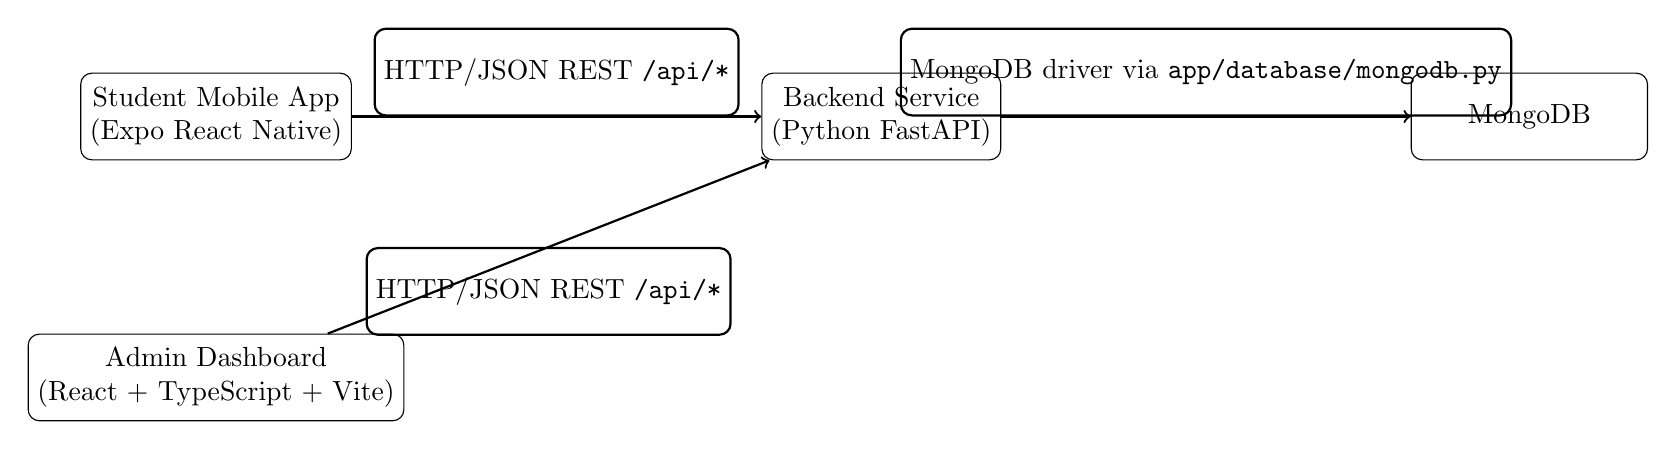
\begin{tikzpicture}[node distance=2.2cm, every node/.style={draw, rounded corners, align=center, minimum width=3cm, minimum height=1.1cm}]
  \node (mobile) {Student Mobile App\\(Expo React Native)};
  \node (admin) [below=of mobile] {Admin Dashboard\\(React + TypeScript + Vite)};
  \node (backend) [right=of mobile, xshift=3cm] {Backend Service\\(Python FastAPI)};
  \node (db) [right=of backend, xshift=3cm] {MongoDB};

  \draw[->, thick] (mobile) -- node[above] {HTTP/JSON REST \texttt{/api/*}} (backend);
  \draw[->, thick] (admin) -- node[below] {HTTP/JSON REST \texttt{/api/*}} (backend);
  \draw[->, thick] (backend) -- node[above] {MongoDB driver via \texttt{app/database/mongodb.py}} (db);
\end{tikzpicture}
\end{center}

\subsection{Backend Module Structure}
The backend is organized into the following functional modules:
\begin{itemize}[nosep]
  \item \texttt{app/main.py}: application startup, CORS, router registration, and health endpoint.
  \item \texttt{app/routes}: REST routers for auth, menu, combos, orders, profile, users, wallet, payments, checkout, QR, and inventory.
  \item \texttt{app/core}: authentication dependencies and security utilities.
  \item \texttt{app/database}: MongoDB connection, collection initialization, and helper functions.
  \item \texttt{app/services}: business logic for orders, wallet, auth, menu, combos, payments, checkout, inventory, and QR generation/verification.
  \item \texttt{app/schemas}: request and response models used for input validation and output serialization.
\end{itemize}

\subsection{Data Flow}
\begin{enumerate}[nosep]
  \item The mobile app performs user authentication via \texttt{POST /api/auth/login} and stores the JWT in AsyncStorage.
  \item User requests from the student app are sent to the backend with the Authorization header attached by \texttt{src/services/api.js}.
  \item The backend resolves user identity via \texttt{app/core/dependencies.py} and accesses MongoDB collections from \texttt{app/database/mongodb.py}.
  \item Orders are created through \texttt{POST /api/orders}, and QR codes are generated through \texttt{GET /api/qr/orders/\{order\_id\}}.
  \item Admin actions traversing \texttt{canteen-admin/src/api/index.ts} call endpoints such as \texttt{GET /api/orders/all}, \texttt{POST /api/menu}, and \texttt{POST /api/inventory}.
\end{enumerate}

\subsection{Security Architecture}
JWT bearer tokens protect most backend endpoints. The backend supports a demo fallback token \texttt{mock-jwt-token} in \texttt{app/core/dependencies.py}. Real authentication uses tokens decoded by \texttt{app/core/security.py} and user retrieval from MongoDB.

\subsection{Deployment Considerations}
The codebase includes separate front-end and backend packages that should be built independently. The mobile app uses a local API base URL configured in \texttt{canteen-frontend/src/services/api.js}. The admin dashboard depends on browser localStorage for admin credentials.


\section{Use Cases}
\label{sec:usecases}
\subsection{Use Case Actors}
\begin{itemize}[nosep]
  \item \textbf{Student User}: uses the mobile app to authenticate, browse food, pay, and track orders.
  \item \textbf{Admin User}: uses the admin dashboard to manage the menu, combos, inventory, orders, and wallet metrics.
\end{itemize}

\subsection{Use Case Diagram}
\begin{center}
\begin{tikzpicture}[node distance=2cm, every node/.style={draw, rounded corners, align=center, minimum width=2.5cm}]
  \node[ellipse] (student) {Student User};
  \node[ellipse, below=of student] (admin) {Admin User};
  \node[rectangle, right=of student, xshift=3cm] (browse) {Browse Menu / Combos};
  \node[rectangle, below=of browse] (order) {Place Order};
  \node[rectangle, below=of order] (wallet) {Wallet Top-Up \& Payment};
  \node[rectangle, below=of wallet] (qr) {Show QR / Verify Order};
  \node[rectangle, right=of admin, xshift=3cm] (manage) {Manage Menu, Combos, Inventory};
  \node[rectangle, below=of manage] (dashboard) {Monitor Orders \& Payments};

  \draw[-] (student) -- (browse);
  \draw[-] (student) -- (order);
  \draw[-] (student) -- (wallet);
  \draw[-] (student) -- (qr);
  \draw[-] (admin) -- (manage);
  \draw[-] (admin) -- (dashboard);
  \draw[-] (admin) -- (order);
\end{tikzpicture}
\end{center}

\subsection{Primary Use Cases}
\subsubsection{UC1: Student Login and Session Restore}
\textbf{Actor}: Student User
\begin{itemize}[nosep]
  \item \textbf{Description}: The mobile app authenticates the student with email and password.
  \item \textbf{Trigger}: User opens the app or submits login form.
  \item \textbf{Preconditions}: User has credentials registered in backend.
  \item \textbf{Main Flow}:
    \begin{enumerate}[nosep]
      \item App sends \texttt{POST /api/auth/login} with credentials.
      \item Backend returns a JWT token and user data.
      \item App stores the token in AsyncStorage and fetches profile via \texttt{GET /api/profile}.
      \item App fetches wallet details via \texttt{GET /api/wallet}.
    \end{enumerate}
  \item \textbf{Postconditions}: User is logged in and redirected to the main app.
\end{itemize}

\subsubsection{UC2: Browse Menu and Add to Cart}
\textbf{Actor}: Student User
\begin{itemize}[nosep]
  \item \textbf{Description}: Student searches and filters menu and combos.
  \item \textbf{Trigger}: User opens the menu screen or selects a category.
  \item \textbf{Main Flow}:
    \begin{enumerate}[nosep]
      \item App calls \texttt{GET /api/menu} with optional filters, or \texttt{GET /api/combos}.
      \item Backend returns available items and combo bundles.
      \item User adds items or combos to cart in the mobile UI.
    \end{enumerate}
  \item \textbf{Postconditions}: Cart state updates in \texttt{CartContext} and user can proceed to checkout.
\end{itemize}

\subsubsection{UC3: Checkout with Wallet or UPI}
\textbf{Actor}: Student User
\begin{itemize}[nosep]
  \item \textbf{Description}: Student completes payment using wallet PIN or UPI.
  \item \textbf{Trigger}: User confims order in cart screen.
  \item \textbf{Main Flow}:
    \begin{enumerate}[nosep]
      \item App optionally requests checkout summary from \texttt{POST /api/checkout/summary}.
      \item App submits \texttt{POST /api/orders} with order details.
      \item If wallet payment is selected, app calls \texttt{POST /api/payments/wallet-pay} with PIN.
      \item If UPI payment is selected, app calls \texttt{POST /api/payments/upi-pay}.
    \end{enumerate}
  \item \textbf{Postconditions}: Order is created, and payment status is returned.
\end{itemize}

\subsubsection{UC4: View Orders and Present QR Code}
\textbf{Actor}: Student User
\begin{itemize}[nosep]
  \item \textbf{Description}: Student views active and completed orders and displays a QR code.
  \item \textbf{Trigger}: User opens the orders screen.
  \item \textbf{Main Flow}:
    \begin{enumerate}[nosep]
      \item App calls \texttt{GET /api/orders}.
      \item App displays active/completed orders and allows order detail navigation.
      \item If available, user taps \textit{Show QR} to present the QR image.
    \end{enumerate}
  \item \textbf{Postconditions}: Student receives current order state and QR for pickup.
\end{itemize}

\subsubsection{UC5: Admin Manage Menu and Combos}
\textbf{Actor}: Admin User
\begin{itemize}[nosep]
  \item \textbf{Description}: Admin performs CRUD operations on menu items and combos.
  \item \textbf{Trigger}: Admin navigates to menu or combos management page.
  \item \textbf{Main Flow}:
    \begin{enumerate}[nosep]
      \item Admin dashboard calls \texttt{GET /api/menu} and \texttt{GET /api/combos}.
      \item Admin submits \texttt{POST /api/menu} or \texttt{POST /api/combos} to create new entries.
      \item Admin edits existing items with \texttt{PATCH /api/menu/\{item\_id\}} or \texttt{PATCH /api/combos/\{combo\_id\}}.
      \item Admin removes items using \texttt{DELETE /api/menu/\{item\_id\}} or \texttt{DELETE /api/combos/\{combo\_id\}}.
    \end{enumerate}
  \item \textbf{Postconditions}: Catalog is updated and reflected in student browsing.
\end{itemize}

\subsubsection{UC6: Admin Inventory and Payment Monitoring}
\textbf{Actor}: Admin User
\begin{itemize}[nosep]
  \item \textbf{Description}: Admin monitors inventory, tracks low-stock items, and views payment metrics.
  \item \textbf{Trigger}: Admin opens inventory or wallet dashboards.
  \item \textbf{Main Flow}:
    \begin{enumerate}[nosep]
      \item Admin dashboard calls \texttt{GET /api/inventory} and \texttt{GET /api/orders/all}.
      \item Admin records inventory receipts via \texttt{POST /api/inventory} or updates records with \texttt{PATCH /api/inventory/\{id\}}.
      \item Admin reviews revenue and transaction summaries in the wallet dashboard.
    \end{enumerate}
  \item \textbf{Postconditions}: Inventory data and payment metrics are kept current in the admin UI.
\end{itemize}


\bibliographystyle{plain}
\bibliography{references}
\end{document}
